% =============================================================
% Chapter 3 --- Tool Calls
% =============================================================

\chapter{Tool Calls}
\label{ch:toolcalls}

\begin{quote}
\itshape
\small
``Large language models are surprisingly good at composing strategies
and surprisingly bad at counting letters. The escape hatch from this
asymmetry is to let the model \emph{call} something that can count.''
\end{quote}

\noindent
This chapter introduces \emph{tool calls} --- the mechanism by which a
language model delegates a sub-task to deterministic, external code and
incorporates the result back into its own reasoning. We argue that
tool calls are not a convenience layer on top of language models but a
\emph{fundamental} extension of their capabilities, lifting them out of
the cognitive cul-de-sacs that pure next-token prediction is known to
fall into. After motivating the topic, we develop tool calls
constructively: starting from a hosted, native API, descending to a
local model that does not know what tool calls are, and ending with
two designs that have come to dominate practice --- a single shell
tool, and a code-execution tool. The chapter closes with the
observation that adding a control loop around tool calls is, in
substance, the move from a chatbot to an agent.

\section{Motivation: The Strawberry Problem}
\label{sec:strawberry}

A reliable way to embarrass a frontier language model is to ask it
how many times the letter \emph{r} occurs in the word
\emph{strawberry}.\footnote{The example dates back to spring 2024 and
has become folklore. Users discovered that successive ``frontier''
releases also failed on minor variants such as \emph{strapberry},
suggesting that the failure is structural, not a particular model's
mistake.}
The correct answer is three. A surprisingly large number of
state-of-the-art models, when asked in plain English, return two.
This is not a sampling fluke and it is not patched by scale: the
failure mode reproduces under temperature zero on small open-weights
models and on the largest hosted ones alike, and it persists on
words the model has demonstrably read thousands of times during
training.

The failure has a clean mechanical explanation. Modern language
models do not see characters; they see \emph{tokens}, which are
typically multi-character substrings produced by a learned subword
tokenizer such as Byte-Pair Encoding. The word \emph{strawberry} is
decomposed by the GPT-4-class tokenizer into roughly three pieces:
\code{st}, \code{raw}, \code{berry}. The model has no first-class
representation of the individual letters that make up those pieces,
and its only access to character-level information is the
correlations the tokens carry from training. \citet{fu2024counting}
show empirically that letter-counting accuracy degrades with the
\emph{frequency} of the word in training corpora and with the
\emph{complexity} of the counting operation, and that the failure is
not removed by chain-of-thought prompting. \citet{xu2024geniusparadox}
make the same point under a different lens: a model that solves
graduate-level mathematics word problems can fail an exercise from
the first week of primary-school spelling, and this is not a
contradiction once we accept that the underlying computation is over
tokens, not letters.

The critical observation, for our purposes, is not that this failure
is surprising. It is that the failure is \emph{trivial to repair} from
outside the model. A three-line Python function counts characters
correctly:

\begin{lstlisting}[language=Python,caption={A reliable letter counter.},label=lst:counter]
def count_letter(word: str, letter: str) -> int:
    return sum(1 for c in word.lower() if c == letter.lower())
\end{lstlisting}

\noindent
A first-week programming exercise solves a problem that the most
expensive language models on Earth get wrong. The correct response
is not to demand that the language model learn to count
letters\footnote{Although several follow-ups~\citep{xu2024geniusparadox}
attempt exactly this, by altering tokenization or by training with
character-level signals.} but to recognise that the language model is
the wrong tool for the job and to give it access to the right one.
This is the core idea of a tool call.

\begin{updatebox}[title={Update --- April 2026}]
\small
The frontier has, somewhat, caught up. In April~2026 OpenAI's
GPT-5.4 announced that the canonical \emph{strawberry} prompt now
returns \emph{three}, and the company circulated the result as
evidence that the underlying reasoning had
improved~\citep{techradar2026strawberry}. Within a day, users
demonstrated that the fix did not generalise: substituting
\emph{cranberry} produced the wrong answer (one ``r'' instead of
three), and adding a deliberate misspelling --- ``how many p's are
in strawpberry?'' --- elicited confidently wrong answers from every
frontier system tested, with several commentators concluding that
the strawberry-specific fix had been
hard-coded~\citep{ninetofivegoogle2026strawberry}. Anthropic's
Claude Opus~4.7~\citep{anthropic2026opus47}, asked the same
misspelled question, produced the answer reproduced in
Figure~\ref{fig:opus47-strawpberry}: it spotted the misspelling but
still miscounted, in the same family of error as the original
strawberry case. The takeaway is not that the frontier still cannot
count letters; the takeaway is that the failure is mechanical, not
adversarial. As long as the model perceives the world as tokens,
point fixes will leak along the seams of those tokens, and the
correct architectural response is the one developed in the rest of
this chapter: give the model a tool that perceives characters.
\end{updatebox}

\begin{figure}[ht]
  \centering
  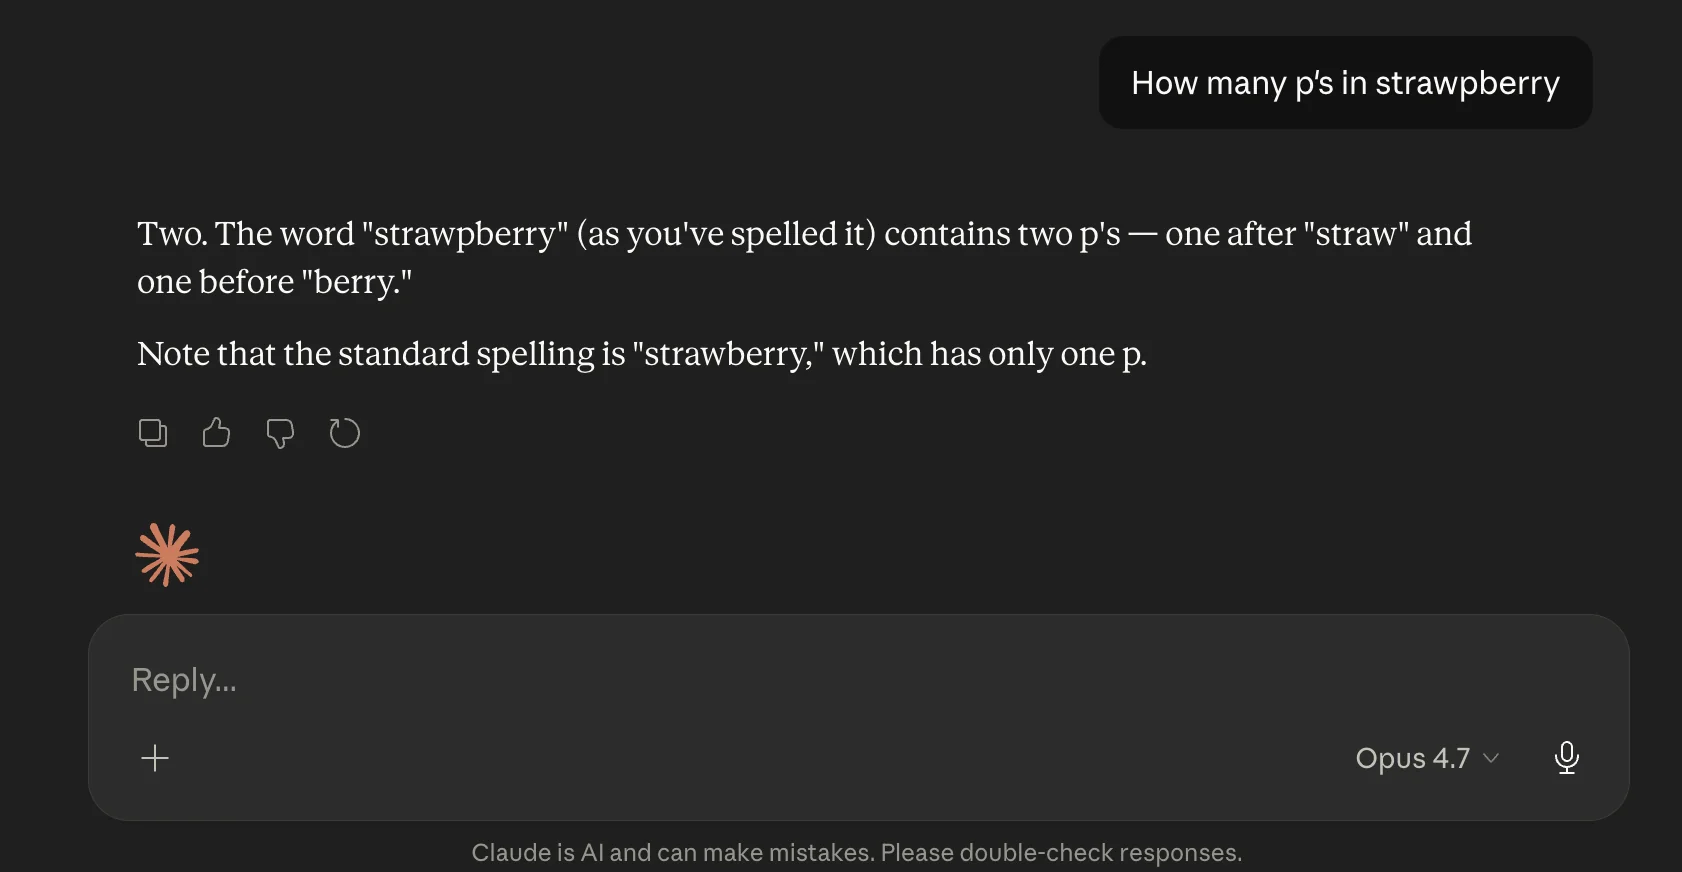
\includegraphics[width=0.78\textwidth]{figures/opus_4_7_strawpberry_fail.png}
  \caption{Claude Opus~4.7 (released 16~April~2026), asked how many
    p's are in the misspelled \emph{strawpberry}, identifies the
    misspelling but still miscounts: the word as spelled contains
    one ``p'', not two. The behaviour is the same family of error as
    the original strawberry case --- an authoritative tone covering
    a tokenizer-level blind spot.}
  \label{fig:opus47-strawpberry}
\end{figure}

\begin{remarkbox}
\small
The strawberry problem is the smallest possible illustration of a
much larger pattern. Pure language models cannot tell the time, do
not know the current weather, cannot retrieve a fresh database row,
and cannot run the code they themselves emit. Each of these is, in
isolation, trivially solved by a few lines of conventional software.
A language model wrapped in a system that lets it \emph{call} that
software is not slightly more capable than the bare model: it is
qualitatively in a different category.
\end{remarkbox}

\section{What Is a Tool Call?}
\label{sec:def}

\begin{definitionbox}
A \textbf{tool call} is a structured, machine-interpretable request,
emitted by a language model in the course of generating a response,
that is intercepted by the surrounding runtime, dispatched to an
external piece of code (the \emph{tool}), and whose result is fed
back into the model's context so generation can continue. A
\textbf{tool} is the external code: a deterministic function with a
declared name, a typed argument schema, and a return value of a type
the model is told it can expect.
\end{definitionbox}

\begin{remarkbox}
\small
A pedantic objection at this point is reasonable: an isolated tool
call --- a single forward pass that emits a structured request --- is
not, on its own, useful. The interesting object is the
\emph{exchange}: question in, tool call out, observation back in,
final answer out. That exchange is already a tiny control loop, and
control loops are the subject matter of the agents chapter. We make
the distinction explicit and stick with it: in this chapter the
``loop'' has a fixed, small upper bound (typically one or two
iterations, just enough to feed the tool result back); a stateful,
goal-driven loop is what turns a tool-using chatbot into an agent
and is treated separately.
\end{remarkbox}

\subsection{Anatomy of a tool-call exchange}
\label{sec:def-exchange}

Before we look at how to implement tool calls, let's walk through an
example with the letter counter tool. We will look at two queries:
\begin{itemize}
\item ``How many r's are in strawberry?''
\item ``What is the capital of Paris?''
\end{itemize}

Figure~\ref{fig:exchange} shows the same flow as a sequence diagram;
the prose below walks through each step.

\begin{figure}[ht]
\centering
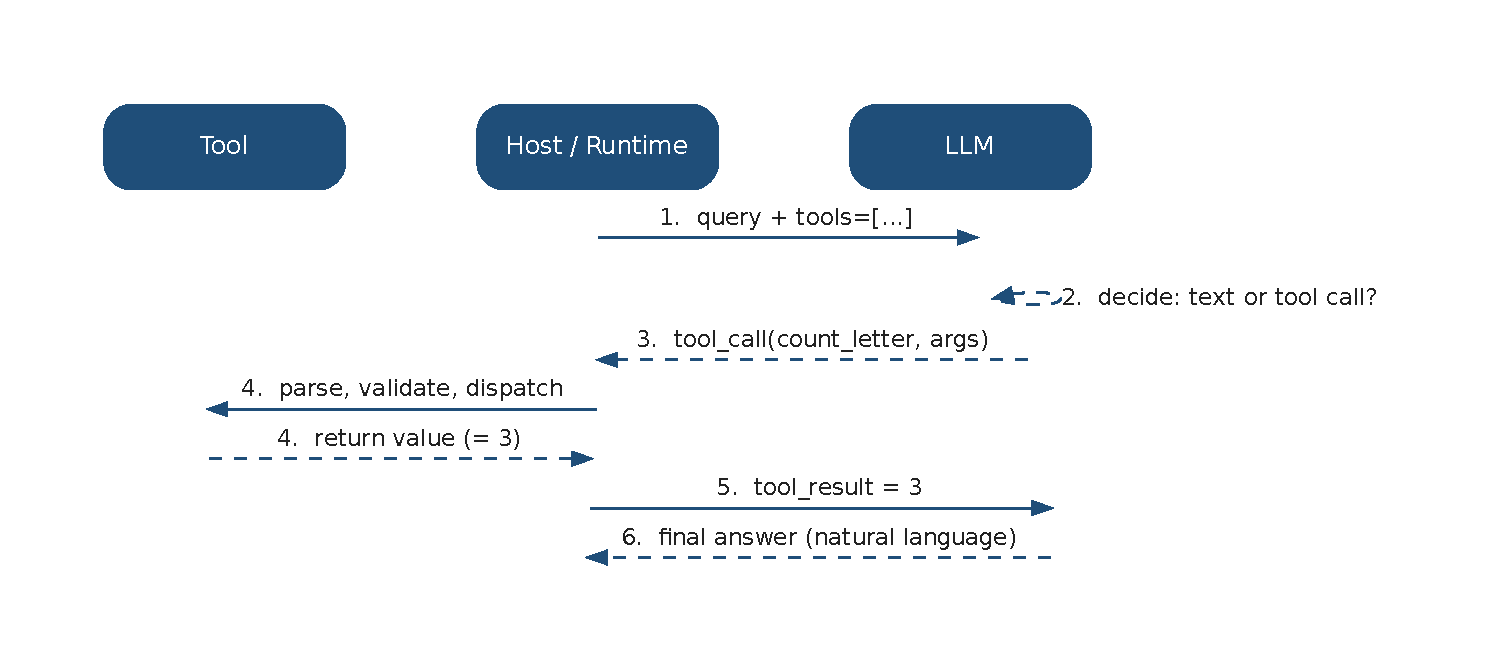
\includegraphics[width=0.95\textwidth]{figures/exchange.pdf}
\caption{Sequence of a tool-call exchange. Time flows top to bottom;
  the row of an arrow corresponds to the step number in the prose.
  Solid arrows are dispatch traffic, dashed arrows are responses on
  their way back. Note that no arrow ever connects \textsf{Tool}
  directly to \textsf{LLM}: the model never talks to a tool without
  going through the runtime, which is what makes the runtime the
  natural place to put parsing, validation, and policy. The diagram
  source lives at \fname{figures/exchange.dot} and is rendered to
  PDF by \code{dot} during the build.}
\label{fig:exchange}
\end{figure}

\begin{enumerate}[label=\textbf{Step \arabic*.},leftmargin=2.3em,itemsep=0.4em]

\item \textbf{Send the query, plus a description of the tools the
  model may use.} Let's have a look at the HTTP request to the model.

\begin{lstlisting}[language=json,caption={The query and tool schema sent to the model.},label=lst:countschema]
{
  "messages": [
    {
      "role": "user",
      "content": "How many r's are in strawberry?"
    }
  ],
  "tools": [
    {
      "name": "count_letter",
      "description": "Count occurrences of a letter in a word.",
      "parameters": {
        "type": "object",
        "properties": {
          "word":   {"type": "string"},
          "letter": {"type": "string", "minLength": 1, "maxLength": 1}
        },
        "required": ["word", "letter"]
      }
    }
  ]
}
\end{lstlisting}

Quite a bit of JSON, but importantly, it separates the user's
  message \emph{and} \code{tools}. The messages struct is self-explanatory,
  the tools struct is a list of tool descriptions, each of which has a name, 
  a natural-language description, and a JSON-schema for its arguments.
  Note what is \emph{not} sent: the actual implementation of
  \code{count\_letter}. The model never sees the Python.

\item \textbf{The model decides whether and how to call the tool.}
  Here the two queries diverge. 
  \begin{itemize}
    \item For the strawberry question, the model emits a
  structured request to call \code{count\_letter} with the appropriate arguments. 
    \item For the Paris question, the model emits a normal text response
  (``Paris is the capital of France'') without calling any tool - as if the 
  tool did not exist. 
  \end{itemize}

  \item \textbf{The model emits the call.} If it chooses to invoke
  \code{count\_letter}, the response is no longer free text. In the
  hosted-API case it is a structured \code{tool\_calls} entry; in the
  plain-text case it is a conventionalised JSON object inside the
  assistant's message. The shape, in both cases, is essentially:

\begin{lstlisting}[language=json]
{"name": "count_letter",
 "arguments": {"word": "strawberry", "letter": "r"}}
\end{lstlisting}

\item \textbf{The runtime parses, extracts, and executes.} 
 Now the runtime examines the answer. Is it a request for a tool call? If not,
 proceed as normal. Render the answer and ask for the next prompt. 
 
 If it is a tool call, which tool and with what arguments? Then, the runtime
 will execute the tool. In our case, it will run the \code{count\_letter} 
 function with the arguments \code{word="strawberry"} and \code{letter="r"}, 
 which will return the integer \code{3}.

\item \textbf{The runtime sends the result back to the model.} Now we 
have to send the result back to the llm. The
  conversation is replayed with one additional turn appended: a
  message of role \code{tool} (or \code{tool\_result}, depending on
  the provider) carrying the value that was returned. Because the
  model is stateless across HTTP requests, this is how it learns
  what its own tool call produced.

\item \textbf{The model produces the final answer.} A second forward
  pass consumes the original user message, the tool advertisement,
  the model's own previous tool-call message, and the new tool-result
  message. With this complete record, the model produces the
  user-facing answer: ``The word \emph{strawberry} contains the
  letter `r' three times.''

\end{enumerate}

\noindent
The structure is six steps, three round-trips of context, and one
piece of Python code. Two of the steps belong to the model
(decisions 2 and 6), three belong to the runtime (1, 4, 5), and one
is the tool itself (the body of step~4). Mixing these up is the
single most common source of confusion when building tool-using
systems.

\begin{remarkbox}
\small
\textbf{Description versus implementation.} The schema in
Listing~\ref{lst:countschema} is what the model sees of the tool;
the Python function in Listing~\ref{lst:counter} is what the runtime
runs. They are not the same artifact and need not even live in the
same process. A tool description is documentation aimed at the
model; a tool implementation is software aimed at the CPU. Treating
them as separate from the start makes everything else cleaner.
\end{remarkbox}

A complete tool-call \emph{transaction} therefore decomposes into
four phases at the level of the runtime --- advertisement, request,
dispatch, continuation --- which are the same four phases that
appear in every concrete API:

\begin{enumerate}[label=(\roman*)]
\item \textbf{Advertisement.} The runtime tells the model which tools
  are available (step~1 above).
\item \textbf{Request.} The model emits a structured request (steps
  2--3).
\item \textbf{Dispatch.} The runtime parses, validates, and executes
  (step~4).
\item \textbf{Continuation.} The runtime appends the result and the
  model produces the answer (steps~5--6).
\end{enumerate}

The distinction between the model's \emph{decision} to call a tool and
the runtime's \emph{execution} of the tool is important and will
recur. In well-designed systems the model does not see the
implementation of any tool; it sees only a name, a docstring-quality
description, and a schema. Conversely, the runtime does not interpret
the model's natural-language reasoning; it only acts on the
structured request. This separation of concerns is what makes the
design scale to dozens or hundreds of tools without leaking
implementation details into the prompt.

\section{A Generic Implementation}
\label{sec:impl}

We now make the four phases of \S\ref{sec:def} executable. We do
this in three passes. First, an LLM-agnostic skeleton that names the
four building blocks every implementation must provide. Second, the
hosted case: OpenAI's Python SDK, where most of the skeleton is
already written. Third, the local case: Gemma~4 served by Ollama,
which has its own native tool-call format and is the model we use
throughout the rest of the book.

A short discussion of what to do when even system-prompting a
non-supporting model fails closes the section.

\subsection{The four building blocks}
\label{sec:impl-blocks}

Independent of which model and which transport are in play, an
implementation of tool calls needs exactly four pieces. Naming them
once, here, makes it easier to read every concrete implementation in
this chapter as a re-encoding of the same skeleton.

\begin{enumerate}[label=\textbf{(\arabic*)},leftmargin=2.2em,itemsep=0.4em]
\item \textbf{A \emph{description} of each tool, addressed to the
  model.} Name, one-paragraph purpose, and a typed argument schema.
  Critically, this is documentation, not code; the model will never
  see the implementation.
\item \textbf{A \emph{registry} mapping tool names to their Python
  implementations.} A plain dictionary suffices. The runtime looks up
  the requested name and invokes the corresponding function.
\item \textbf{A \emph{parser} that turns the model's response into a
  list of tool calls (or recognises that there are none).} What
  ``response'' means depends on the transport: a structured field on
  hosted APIs, a substring of free-form text on local models. The
  parser is the most failure-prone component on non-native models
  and the most invisible component on native ones.
\item \textbf{A \emph{loop} that ties them together.} While the model
  asks for tool calls, dispatch them, append the results to the
  conversation, and ask the model to continue. Stop when the model
  produces a normal text reply. Cap the iteration count.
\end{enumerate}

In pseudocode the loop is six lines:

\begin{lstlisting}[language=Python,caption={LLM-agnostic skeleton of a tool-calling client.},label=lst:skeleton]
def query(user_message, tool_descriptions, tool_registry,
          parser, send_to_llm, max_steps=4):
    messages = [{"role": "user", "content": user_message}]
    for _ in range(max_steps):
        reply       = send_to_llm(messages, tool_descriptions)
        tool_calls  = parser(reply)
        messages.append(reply)
        if not tool_calls:
            return reply["content"]                # final answer
        for call in tool_calls:
            result = tool_registry[call.name](**call.args)
            messages.append({"role": "tool",
                             "name":  call.name,
                             "content": json.dumps(result)})
    raise RuntimeError("tool-call loop exceeded max_steps")
\end{lstlisting}

\noindent
The two implementations that follow differ in only two of the
arguments: \code{send\_to\_llm} (which provider, which transport) and
\code{parser} (how to recover structured calls from the response).
\code{tool\_descriptions} and \code{tool\_registry} stay the same.

\subsection{Native function calling: the hosted case}
\label{sec:impl-hosted}

Major providers (OpenAI, Anthropic, Google) have converged on the
same shape of
API~\citep{openai2024functioncalling,anthropic2024toolusage}: the
caller declares tools using a JSON-schema for arguments; the provider
returns either a textual message or a structured \code{tool\_calls}
field; the caller executes the tool and posts the result back as a
\code{tool\_result} message. The dispatcher and loop reduce to a few
lines because the SDK is doing the parsing for us.

\begin{lstlisting}[language=Python,caption={The shortest end-to-end tool call against a hosted provider.},label=lst:openai]
from openai import OpenAI
import json

# Building block 1: tool description (sent to the LLM).
TOOLS = [{
    "type": "function",
    "function": {
        "name": "count_letter",
        "description": "Count how many times a letter occurs in a word.",
        "parameters": {
            "type": "object",
            "properties": {
                "word":   {"type": "string"},
                "letter": {"type": "string", "minLength": 1, "maxLength": 1},
            },
            "required": ["word", "letter"],
        },
    },
}]

# Building block 2: the implementations and a name -> function registry.
def count_letter(word: str, letter: str) -> int:
    return sum(1 for c in word.lower() if c == letter.lower())

DISPATCH = {"count_letter": count_letter}

# Building block 3: parsing is done for us by the SDK; tool_calls is a
# structured field on the response message.

# Building block 4: the loop.
def query(user_message: str, model: str = "gpt-4o-mini",
          max_steps: int = 4) -> str:
    client   = OpenAI()
    messages = [{"role": "user", "content": user_message}]
    for _ in range(max_steps):
        rsp = client.chat.completions.create(
            model=model, messages=messages, tools=TOOLS,
        )
        msg = rsp.choices[0].message
        messages.append(msg)
        if not msg.tool_calls:
            return msg.content
        for call in msg.tool_calls:
            args   = json.loads(call.function.arguments)
            result = DISPATCH[call.function.name](**args)
            messages.append({
                "role":         "tool",
                "tool_call_id": call.id,
                "content":      json.dumps(result),
            })
    raise RuntimeError("tool-call loop exceeded max_steps")


if __name__ == "__main__":
    print(query("How many r's are in 'strawberry'?"))
\end{lstlisting}

\noindent
Three things are worth pointing out. First, the tool is a perfectly
ordinary Python function: nothing about it is model-aware. The schema
in \code{TOOLS} is the only place where the model and the function
meet. Second, the loop is bounded but otherwise unconditional: a
model is allowed to issue several tool calls back-to-back, and the
runtime keeps cycling until the model emits a regular text response
or \code{max\_steps} is exhausted. Third, the model's output when it
issues a tool call is not free-form text; the SDK has already parsed
it into the \code{tool\_calls} field on the response.

\subsection{Native tool calling on Ollama: the Gemma~4 case}
\label{sec:impl-gemma}

Gemma~4 ships with native tool calling.\footnote{Released
2~April~2026; documented at
\href{https://ai.google.dev/gemma/docs/capabilities/text/function-calling-gemma4}{ai.google.dev/gemma/docs/capabilities/text}.}
The model's underlying chat template wraps tool declarations in a
dedicated \code{<\,|tool>~\dots~<tool|>} block and emits requests
inside \code{<\,|tool\_call>~\dots~<tool\_call|>} tags;
the host is expected to inject the result inside
\code{<\,|tool\_response>~\dots~<tool\_response|>} before the model
produces its final answer. The full template is reproduced
in~\citet{gemma4card}.

The good news is that we almost never need to manipulate those
tokens directly. Ollama's \code{/api/chat} endpoint accepts the
same JSON-schema tool descriptions as OpenAI's API, applies Gemma~4's
native template internally, and parses the result back into a
structured \code{tool\_calls} field on the assistant message. From
the application's point of view the only differences from
Listing~\ref{lst:openai} are the URL we POST to and the assistant
message format.

\begin{lstlisting}[language=Python,caption={Native tool calling against a local Gemma~4 served by Ollama.},label=lst:gemma]
import json
import requests

OLLAMA_URL = "http://192.168.50.3:11700/api/chat"
MODEL      = "gemma4:26b"

# Building block 1: tool description (same JSON-schema as in Listing 3.2).
TOOLS = [{
    "type": "function",
    "function": {
        "name": "count_letter",
        "description": "Count occurrences of a letter in a word.",
        "parameters": {
            "type": "object",
            "properties": {
                "word":   {"type": "string"},
                "letter": {"type": "string", "minLength": 1, "maxLength": 1},
            },
            "required": ["word", "letter"],
        },
    },
}]

# Building block 2: implementation + registry.
def count_letter(word: str, letter: str) -> int:
    return sum(1 for c in word.lower() if c == letter.lower())

DISPATCH = {"count_letter": count_letter}

# Building block 3: the response.message.tool_calls field on Ollama is
# already a list of {"function": {"name", "arguments"}} dicts.

# Building block 4: the loop.
def query(user_message: str, model: str = MODEL,
          max_steps: int = 4) -> str:
    messages = [{"role": "user", "content": user_message}]
    for _ in range(max_steps):
        rsp = requests.post(OLLAMA_URL, json={
            "model":    model,
            "stream":   False,
            "messages": messages,
            "tools":    TOOLS,
        }, timeout=120)
        rsp.raise_for_status()
        msg = rsp.json()["message"]
        messages.append(msg)
        tool_calls = msg.get("tool_calls") or []
        if not tool_calls:
            return msg.get("content", "")
        for call in tool_calls:
            name = call["function"]["name"]
            args = call["function"]["arguments"]
            if isinstance(args, str):           # some Ollama builds stringify
                args = json.loads(args)
            result = DISPATCH[name](**args)
            messages.append({
                "role":    "tool",
                "name":    name,
                "content": json.dumps(result),
            })
    raise RuntimeError("tool-call loop exceeded max_steps")


if __name__ == "__main__":
    print(query("How many r's are in 'strawberry'?"))
\end{lstlisting}

\noindent
The runnable script accompanying this listing
(\fname{manuscript/scripts/gemma4\_native\_toolcall.py}) prints the
raw assistant message in addition to the parsed answer, so the reader
can confirm what Gemma~4 actually emitted under Ollama's hood. The
shape of \code{messages} after a successful exchange will be: user
message, assistant message with a \code{tool\_calls} field and an
empty \code{content}, tool-result message, assistant message with
the final answer.

\subsection{No native support: prompting a model that does not know the format}
\label{sec:impl-fallback}

Until very recently, ``no native tool-call channel'' described much
of the open-weights ecosystem; even today it describes most small
models. The construction in this case is to \emph{prompt} the model
into structured output: instruct it, in the system prompt, to emit
JSON of a specified shape and nothing else when it intends to call a
tool, and then parse the model's free-form text yourself. We do not
work this out in full code here --- the result is a longer version
of Listing~\ref{lst:gemma} with a regular-expression parser
substituted for the structured \code{tool\_calls} field --- but the
shape of the system prompt is worth showing:

\begin{lstlisting}[caption={Fragment of a system prompt that elicits structured tool calls from a model with no native support.},label=lst:fallback-prompt]
You are a helpful assistant with access to one tool:

  count_letter(word: str, letter: str) -> int
    Returns the number of times `letter` occurs in `word`.

To use the tool, respond with EXACTLY a JSON object on a single
line, and NOTHING ELSE -- no prose, no code fences:
  {"tool": "count_letter", "args": {"word": "...", "letter": "..."}}

When the system has the tool's answer, the user message will append:
  TOOL_RESULT: <value>
After that, respond to the user normally.
\end{lstlisting}

\noindent
Four practical observations carry over from this construction even
though we do not give a runnable example for it:

\begin{enumerate}[label=(\arabic*)]
\item \textbf{Format discipline lives in the system prompt.} The
  exact JSON shape, the prohibition on prose, and the convention for
  the result are all communicated through natural language. The
  reliability of the loop is bounded above by how strictly the model
  follows that format.
\item \textbf{Parsing must be defensive.} Models occasionally wrap
  the JSON in markdown fences, append a trailing
  \emph{``This will count the r's in strawberry.''}, or hallucinate a
  closing quote. A tolerant regex plus a soft-recovery branch (``your
  JSON was malformed, please re-emit'') is the minimum.
\item \textbf{Few-shot examples are usually necessary.} The system
  prompt can be made shorter and the model more obedient by including
  one or two worked examples of the desired format.
\item \textbf{The cap on iterations is non-negotiable.} Malformed-JSON
  loops can consume an unbounded amount of context and money.
\end{enumerate}

The general topic --- how to coax a model into emitting any
structured output reliably --- is the subject of
\S\ref{sec:structured} in Chapter~\ref{ch:fundamentals} on LLM
fundamentals; tool calling is the most prominent application of it.
When prompting alone is not enough, three escape hatches are common
in practice: switch to a constrained-generation backend
(\code{llama.cpp} grammars, \code{Outlines},
\code{lm-format-enforcer}), which forces the model to emit only
tokens consistent with a JSON-schema; \emph{train} the model to emit
a tool-call format, as \citet{schick2023toolformer} do; or feed the
model's free-form response through a smaller, well-trained parser
model that converts intent into a structured call. Each reduces the
burden on the front-line model at the cost of deployment complexity.

\section{A Taxonomy of Common Tool Calls}
\label{sec:taxonomy}

Tool calls began as a way around the strawberry-style limitations of
language models, but the design generalised quickly. The tools
deployed in production fall into a small number of families. We list
them roughly in order of how strongly they extend the model's
abilities.

\begin{description}[style=nextline,leftmargin=1.5em]
\item[Closed-form computation.] Calculators, unit conversion,
  letter-counting, regex matchers, date arithmetic, evaluation of
  chemical formulae. The defining property is that the right answer
  is determined by the inputs and is checkable. These tools repair
  failures of the strawberry kind.
\item[Real-world state.] The current time, the current weather, the
  current price of a stock, the contents of a user's calendar. These
  tools repair the model's frozen world view: a 2025 model in 2026
  cannot know who won yesterday's election but can be told.
\item[Information retrieval.] Web search, database queries,
  vector-store retrieval, internal corpora. The boundary between
  ``retrieval-augmented generation'' (RAG) and a tool call is
  largely about \emph{who} decides when to retrieve: the runtime in
  RAG, the model in a tool-calling design.
\item[Action in external systems.] Sending an e-mail, opening a pull
  request, paying an invoice, filing a bug. These tools change
  external state and require a different threat model from the
  passive ones above. We return to this in \S\ref{sec:shell}.
\item[Specialised models.] Image generation, image understanding,
  speech transcription, code interpreter, and protein structure
  prediction are all routinely exposed as tool calls. The
  ``language'' model becomes a meta-controller routing requests to
  domain-specialised submodels~\citep{patil2023gorilla}.
\end{description}

\noindent
A useful empirical observation: the value of a tool to a language
model is rarely proportional to its complexity. The strawberry
counter is a few lines and adds an entire category of correctness;
the most sophisticated retrieval system in the world is dominated, in
end-user experience, by whether the model decides to call it at the
right moment. Section~\ref{sec:shell} pushes this observation to its
extreme.

\subsection{Worked examples, one per family}
\label{sec:taxonomy-examples}

The categories above are easier to internalise alongside concrete
tool descriptions. The five examples that follow are deliberately
trimmed --- we give just enough of the schema to make the call site
unambiguous --- so they can be read in sequence.

\begin{description}[style=nextline,leftmargin=1.5em]

\item[Closed-form: \code{count\_letter}.] The strawberry counter we
  have used throughout this chapter. Two strings in, one integer out,
  no side effects. The tool description is Listing~\ref{lst:countschema}.

\item[Real-world state: \code{get\_current\_weather(location:~str)}.]
  Returns a JSON object \code{\{"temperature\_c", "conditions",
  "as\_of"\}} for the requested place. Side-effect-free, but the
  return value is non-deterministic across time. A good default
  testbed for any new agent: it is a one-line API wrapper, but it
  forces the harness to handle network errors gracefully.

\item[Information retrieval: \code{web\_search(query:~str,
  k:~int=5)}.] Returns a list of search results
  \code{[\{"title", "url", "snippet"\}]}. \emph{Web search deserves
  special mention as the single most powerful tool one can give a
  language model.} It cuts directly across the
  ``frozen world view'' and ``no fresh facts'' limitations and
  composes well with code execution: an agent can search, fetch,
  parse, and reason in one loop. Almost every contemporary
  general-purpose assistant exposes some form of it, and a usable
  open-weights agent on commodity hardware becomes dramatically more
  capable the moment a search tool is wired in.

\item[Action: \code{send\_email(to:~str, subject:~str, body:~str)}.]
  Returns a delivery receipt; sends an email as a side effect. From
  the model's point of view this is a tool call like any other, but
  from the system's point of view it crosses an important line: the
  result of the call cannot be undone. Confirmation prompts, dry-run
  modes, and capability gates (\S\ref{sec:sandbox}) live around tools
  of this family.

\item[Specialised model: \code{transcribe\_audio(path:~str)}.] Returns
  a transcript string. Internally the tool runs a Whisper-class
  speech-to-text model. From the LLM's perspective this is opaque ---
  it sees one schema and one return type --- but the call hides a
  multi-billion-parameter network. \citet{patil2023gorilla} treat
  this routing pattern as the central design problem of agents that
  span multiple specialised models.

\end{description}

The five examples cover the categories of the previous list with one
artefact each. A larger production system typically exposes one or
two from each family; the numbers we have seen in practice rarely
exceed twenty before the model's ability to choose the right tool
becomes the bottleneck rather than the inventory.

\section{The Shell as a Tool}
\label{sec:shell}

The previous section listed tools by family. There is a complementary
view, which is to ask: \emph{what is the smallest set of tools that
can do almost everything?} On a Unix system, the answer is one tool:
a shell.

A bash tool is a function with one argument, a command string, that
returns the command's standard output, standard error, and exit
code. It is six lines of code. With access to it, a language model
can:

\begin{itemize}[leftmargin=1.5em,topsep=0.2em,itemsep=0.1em]
\item Read and write files (\code{cat}, \code{tee}, \code{sed}).
\item Search a codebase (\code{grep}, \code{rg}, \code{find}).
\item Run unit tests, linters, type-checkers, and the build system.
\item Execute Python or any other interpreter inline
  (\code{python3 -c "..."}).
\item Talk to the network (\code{curl}, \code{wget}).
\item Interact with version control (\code{git}).
\item Inspect or modify the environment (\code{ps}, \code{kill},
  \code{export}).
\item Install software it decides it needs (\code{pip},
  \code{apt-get}).
\end{itemize}

The breadth of this is hard to overstate, and it is one of the
defining design decisions of contemporary coding agents. The Claude
Code system, for example, treats a constrained shell tool as the
\emph{spine} of the agent and adds higher-level affordances (file
read, edit, write) only as ergonomics on top of it~\citep{liu2026claudecode}.

\begin{examplebox}
\small
\textbf{Implementing the strawberry counter via a shell.} An agent
with only a bash tool can solve the strawberry problem without a
purpose-built counter:

\begin{lstlisting}[language=bash]
$ python3 -c "print('strawberry'.count('r'))"
3
\end{lstlisting}

\noindent
The model wrote the Python; bash executed it; the answer travelled
back as a tool result. The same loop, with longer programs, suffices
for most software-engineering tasks.
\end{examplebox}

\begin{examplebox}
\small
\textbf{Two-step: write a script, then run it.} For anything beyond
a one-liner the agent splits the work into two shell calls. First it
writes a file using a heredoc; then it executes that file. A typical
exchange to count letters across many words looks like:

\begin{lstlisting}[language=bash,caption={First shell call --- create a script file.}]
$ cat > /tmp/count_many.py <<'PY'
import sys
words = sys.argv[1].split(",")
for w in words:
    print(f"{w}: {w.count('r')}")
PY
\end{lstlisting}

\begin{lstlisting}[language=bash,caption={Second shell call --- execute the script.}]
$ python3 /tmp/count_many.py "strawberry,cranberry,blueberry"
strawberry: 3
cranberry: 3
blueberry: 2
\end{lstlisting}

\noindent
Three observations. First, the model has now produced \emph{and}
inspected its own code; if the script crashes, the next iteration of
the loop sees the traceback and can repair the script. Second, the
file persists between shell calls --- the working directory is part
of the agent's state --- so a longer task can build up a small
codebase across many turns. Third, this is the smallest possible
example of an agent that \emph{programs}: the action space includes
authoring artefacts, not just invoking pre-built tools.
\end{examplebox}

\subsection{Risks and sandboxing}
\label{sec:sandbox}

A bash tool with no constraints is also the largest blast radius an
agent can have. The same primitives that let the model fix a bug let
it delete the user's home directory, exfiltrate secrets through
\code{curl}, or install a backdoor. There are several well-documented
incident classes:

\begin{enumerate}[label=(\arabic*)]
\item \textbf{Honest mistakes.} The model issues
  \code{rm -rf build/} and a path expansion expands \code{build} to
  the empty string.
\item \textbf{Prompt injection.} A page the agent fetches contains
  instructions hidden in HTML comments that tell the model to
  \code{cat \~{}/.ssh/id\_rsa | curl}.
\item \textbf{Confused-deputy attacks.} The model has more authority
  than the user who instructed it (e.g.\ a CI runner) and is asked,
  through a comment in a pull request, to use that authority for
  the attacker.
\item \textbf{Quiet system pollution.} Even without any malicious
  input, the agent will cheerfully \code{pip install} a half-dozen
  packages it decided it needed, upgrade a globally installed CLI to
  a newer major version because the older one ``does not support
  the flag I want'', or write configuration files into the user's
  home directory. None of these is catastrophic on their own; over
  hundreds of agent turns they accumulate into an environment the
  user no longer recognises.
\end{enumerate}

\begin{warningbox}
\small
A shell tool should never be exposed to a language model on a
machine the developer cares about. The minimum baseline is to run
the shell inside a container with: a) no access to host
filesystems beyond a designated working directory, b) a network
allow-list rather than full Internet access, c) a CPU/memory/time
budget enforced by the kernel, and d) ephemeral state that is
discarded between sessions. Beyond Docker~\citep{docker2013}, the
options include user-mode kernels such as
gVisor~\citep{gvisor2018}, lightweight seccomp profiles such as
Firejail~\citep{firejail}, and full virtual machines.
\end{warningbox}

\noindent
Two practical recommendations follow from the list above and from
hard-won operational experience. They are stacked, not alternatives:
each addresses a different failure mode.

\begin{enumerate}[label=\textbf{(\arabic*)},leftmargin=2.2em,itemsep=0.4em]

\item \textbf{Sandbox the agent's environment.} The
  \emph{security-critical} risks --- (1) through (3) above --- are
  what motivates sandboxing in the literature, but the
  \emph{day-to-day} payoff is class~(4): an ephemeral, scoped
  environment makes ``the agent installed Python 3.13 over my
  Python~3.11'' simply impossible. Whatever the agent does inside
  the sandbox is thrown away at the end of the session. The
  developer's own toolchain is untouched.

\item \textbf{Run the agent on version-controlled files.} Even with
  a perfect sandbox, the artefacts the agent produces (and edits,
  and \emph{re-edits}) live somewhere. If those files are tracked by
  a version-control system --- ideally with a fresh branch per agent
  session --- every change becomes inspectable, blamable, and
  trivially reversible. \code{git diff} between two agent turns is
  the most-useful single signal we have found for debugging an
  agent's behaviour. Note the qualification: the agent itself can in
  principle rewrite history (\code{git reset --hard},
  \code{git push --force}), so the version-control host should sit
  outside the sandbox or be a remote the sandbox has no credentials
  to push to. Pushed against the right ratchet, version control
  turns the agent's output from an opaque side-effect on the file
  system into an auditable patch series.

\end{enumerate}

\noindent
Sandboxing is the engineering price of the shell-as-spine design. It
is paid once and amortised across every tool the model might want to
add later: an agent that has a shell does not need a separate
``write file'' tool, a separate ``run tests'' tool, or a separate
``install dependency'' tool, because the shell already provides all
three.

\section{Code as the Universal Action}
\label{sec:codeact}

The shell tool of \S\ref{sec:shell} is one specialisation of a more
general design principle: the model's action space should be a
\emph{programming language}. \citet{wang2024codeact} make the
argument explicitly. They propose \emph{CodeAct}, in which the agent
emits Python instead of JSON tool calls; the runtime executes the
Python in a stateful interpreter; and the result --- standard
output, exceptions, returned values --- is fed back. They report
substantial gains on agent benchmarks against the JSON-tool-call
baseline, and trace the gains to two structural properties:

\begin{itemize}[leftmargin=1.5em]
\item \textbf{Composition.} A single Python turn can compose several
  ``tools'' into one expression --- iterate over a list, transform
  each element, sort, slice. With JSON tool calls this requires one
  call per primitive, with the resulting state stored in conversation
  history.
\item \textbf{Library access.} Anything available to the
  interpreter --- \code{numpy}, \code{requests}, an in-process
  vector store, the user's own Python helpers --- is available to
  the model without per-tool schema work.
\end{itemize}

\citet{liang2023codeaspolicies} arrive at the same conclusion in
embodied robotics: programs, not commands, are the natural action
representation when the action space is rich. Anthropic's
\emph{Code execution with MCP} guidance generalises the design to
the Model Context Protocol~\citep{mcp2024spec,anthropic2025mcpcode}:
instead of advertising hundreds of fine-grained tools, an MCP server
exposes a code-execution endpoint, and individual operations become
imports inside the executed code. The transcript shrinks
dramatically and the model gets to plan multi-step operations as a
single program.

We refer to designs of this family --- where the agent's primary
output is a program rather than a sequence of structured calls --- as
\emph{programmatic tool calling}. They subsume the JSON-tool-call
design (a single function call is a program of length one) and
inherit the safety profile of the shell tool: anything dangerous in
\S\ref{sec:sandbox} applies, in stronger form, here.

\begin{remarkbox}
\small
There is a striking asymmetry between what language models are
\emph{good at} producing and what they have historically been
\emph{asked to} produce. Models are extremely strong at writing
code; they are merely adequate at producing well-formed JSON. The
JSON-tool-call interface was an accident of history: it was the
shape providers built first because it was the shape that fits the
existing function-call abstractions in the underlying SDKs. The
programmatic-tool-call shape aligns the interface with the model's
strengths. We expect this trend to continue: future agent harnesses
will treat code execution, not JSON dispatch, as the default
mechanism for action.
\end{remarkbox}

\section{Outlook: Tool Calls as the Gateway to Agents}
\label{sec:agents}

We have so far described tool calls as a static facility: the model
issues a request, the tool answers, the conversation continues. The
move from this to \emph{agents} is, on the surface, a small one. We
take the tool-calling loop of \S\ref{sec:def} and make it
\emph{stateful}, \emph{multi-step}, and \emph{driven by the model's
own goals} rather than by a single user message. Agents add three
things on top of the tool-call substrate:

\begin{enumerate}[label=(\roman*)]
\item \textbf{A control loop.} The model keeps issuing tool calls
  until it judges the task complete; the runtime drives the loop.
\item \textbf{Reasoning interleaved with action.} Each step
  alternates between a thought and an action, in the pattern made
  popular by ReAct~\citep{yao2023react}.
\item \textbf{An evolving context.} The accumulated tool results
  become a working memory that has to be curated to remain useful;
  recent work~\citep{zhang2025ace} treats this curation as a
  first-class concern.
\end{enumerate}

\noindent
Each of these is a chapter of its own. The point we want to make
here, before moving on, is that the substrate they all build on is
the tool call. If the JSON parser of \S\ref{sec:impl} is unreliable,
no amount of clever planning will rescue the agent. If the shell
sandbox of \S\ref{sec:shell} leaks, no amount of evolving context
will undo the damage.
\citet{wang2024codeact}'s subtitle, ``Executable Code Actions Elicit
Better LLM Agents'', is the natural transition into the next
chapter. The substrate determines the ceiling.

\section*{Further Reading}
\addcontentsline{toc}{section}{Further Reading}

\citet{schick2023toolformer} is the canonical reference for
self-supervised training to use tools. \citet{yao2023react}
introduces the reasoning-action interleaving pattern that almost
every subsequent agent inherits. \citet{patil2023gorilla} is the
right starting point for tool calls at the scale of thousands of
APIs. \citet{wang2024codeact} and \citet{anthropic2025mcpcode} are
the foundational pieces for the programmatic-tool-call design.
\citet{fu2024counting} and \citet{xu2024geniusparadox} document the
strawberry phenomenon at the level a textbook reader will want.
\citet{liu2026claudecode} provides a detailed system-design study of
a deployed coding agent built almost entirely on top of a shell
tool, and is recommended reading before designing one's own agent
harness.
